\documentclass[tikz,border=10pt]{standalone}
\usetikzlibrary{calc}
\begin{document}
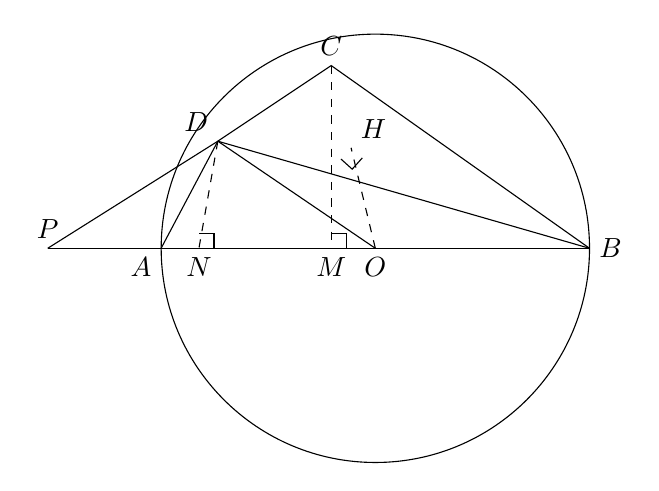
\begin{tikzpicture}[scale=1.6]
\coordinate (O) at (0,0);
\coordinate (A) at (-1.7,0);
\coordinate (B) at (1.7,0);
\coordinate (P) at (-2.6,0);
\coordinate (N) at (-1.4,0);
\coordinate (D) at (-1.25,0.85);
\coordinate (M) at (-0.35,0);
\coordinate (C) at (-0.35,1.45);
\coordinate (H) at ($(O)!0.55!(C)$);

\draw (O) circle (1.7);
\draw (P) -- (B);
\draw (P) -- (D) -- (B);
\draw (D) -- (C) -- (B);
\draw (A) -- (D);
\draw (D) -- (O);
\draw[dashed] (D) -- (N);
\draw[dashed] (C) -- (M);
\draw[dashed] (O) -- (H);

\draw ($(N)+(0.12,0)$) -- ($(N)+(0.12,0.12)$) -- ($(N)+(0,0.12)$);
\draw ($(M)+(0.12,0)$) -- ($(M)+(0.12,0.12)$) -- ($(M)+(0,0.12)$);
\draw[rotate around={48:(H)}] ($(H)+(-0.12,0)$) -- ($(H)+(-0.12,-0.12)$) -- ($(H)+(0,-0.12)$);

\foreach \p/\pos in {P/above, A/below left, N/below, D/above left, C/above, M/below, O/below, B/right, H/above right}
  \node[\pos] at (\p) {$\p$};
\end{tikzpicture}
\end{document}
